%---------- COURSE INFORMATION ------------------------
\newcommand{\course}{CS 490-02}
\newcommand{\coursetitle}{Indepedent Study - Advanced Topics in Programming}
\newcommand{\courseloc}{N/A}
\newcommand{\coursetime}{N/A}
\newcommand{\coursedesc}{Computing topics selected according to the needs of the students.}

\newcommand{\coursesec}{01}
\newcommand{\coursecredithours}{3}
\newcommand{\courseprereq}{Departmental approval.}
\newcommand{\coursedelmethod}{Individual instruction}

\newcommand{\courseobjectives}{\item Explain the use of 3D printing in Human-Computer Interaction
	\item Create a usable interface to monitor and control 3D printers from a cloud-based server
	\item Explain the process of building a 3D printing farm.
}

\newcommand{\coursetopics}{\item 3D Printing for Rapid Prototyping
	\item 3D Printer Building
	\item Cloud-based 3D printing and monitoring
}
\newcommand{\coursegrades}{Project Work\dotfillsmall 30\% \\
		Final Presentation and Paper\dotfillsmall 70\% }
\newcommand{\coursetext}{
   No printed textbook required. Various online readings and research.
%	\adjustbox{valign=c}{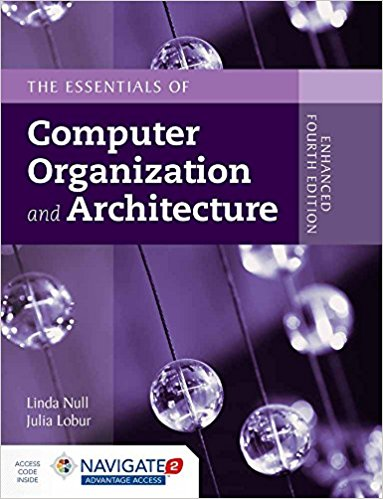
\includegraphics[width=1in]{img/cs490}} & \hangindent .4in \textbf{Textbook:} Null, L., Lobur, J. (2015). Essentials of Computer Organization and Architecture (4th edition). Jones \& Bartlett Learning. ISBN-10: 128407448X, ISBN-13: 978-1284074482. \\
	%& \hangindent .4in Simulation Software: SAM 365 \& 2016 Assessments, Trainings, and Projects with MindTap Reader.
}